%%%%%%%%%%%%%%%%%%%%%%%%%%%%%%%%%%%%%%%%%
% Beamer Presentation
% LaTeX Template
% Version 1.0 (10/11/12)
%
% This template has been downloaded from:
% http://www.LaTeXTemplates.com
%
% License:
% CC BY-NC-SA 3.0 (http://creativecommons.org/licenses/by-nc-sa/3.0/)
%
%%%%%%%%%%%%%%%%%%%%%%%%%%%%%%%%%%%%%%%%%

%----------------------------------------------------------------------------------------
%	PACKAGES AND THEMES
%----------------------------------------------------------------------------------------

\documentclass[xcolor={table}]{beamer}
%\documentclass[notes=only,xcolor={table}]{beamer} % Use this option to generate note slides

\usepackage{algorithm2e}

%\SetAlgoCaptionSeparator{.\space}
%\renewcommand\AlCapFnt{\normalfont\scshape}

\mode<presentation> {

% The Beamer class comes with a number of default slide themes
% which change the colors and layouts of slides. Below this is a list
% of all the themes, uncomment each in turn to see what they look like.

%\usetheme{default}
%\usetheme{AnnArbor}
%\usetheme{Antibes}
%\usetheme{Bergen}
%\usetheme{Berkeley}
\usetheme{Berlin}
%\usetheme{Boadilla}
%\usetheme{CambridgeUS}
%\usetheme{Copenhagen}
%\usetheme{Darmstadt}
%\usetheme{Dresden}
%\usetheme{Frankfurt}
%\usetheme{Goettingen}
%\usetheme{Hannover}
%\usetheme{Ilmenau}
%\usetheme{JuanLesPins}
%\usetheme{Luebeck}
%\usetheme{Madrid}
%\usetheme{Malmoe}
%\usetheme{Marburg}
%\usetheme{Montpellier}
%\usetheme{PaloAlto}
%\usetheme{Pittsburgh}
%\usetheme{Rochester}
%\usetheme{Singapore}
%\usetheme{Szeged}
%\usetheme{Warsaw}

% As well as themes, the Beamer class has a number of color themes
% for any slide theme. Uncomment each of these in turn to see how it
% changes the colors of your current slide theme.

%\usecolortheme{albatross}
\usecolortheme{beaver}
%\usecolortheme{beetle}
%\usecolortheme{crane}
%\usecolortheme{dolphin}
%\usecolortheme{dove}
%\usecolortheme{fly}
%\usecolortheme{lily}
%\usecolortheme{orchid}
%\usecolortheme{rose}
%\usecolortheme{seagull}
%\usecolortheme{seahorse}
%\usecolortheme{whale}
%\usecolortheme{wolverine}

%\setbeamertemplate{footline} % To remove the footer line in all slides uncomment this line
\setbeamertemplate{footline}[page number] % To replace the footer line in all slides with a simple slide count uncomment this line

\setbeamertemplate{navigation symbols}{} % To remove the navigation symbols from the bottom of all slides uncomment this line
}

\usepackage{graphicx} % Allows including images
\usepackage{booktabs} % Allows the use of \toprule, \midrule and \bottomrule in tables

%----------------------------------------------------------------------------------------
%	TITLE PAGE
%----------------------------------------------------------------------------------------

\title[A GP Approach to QoS-Aware Web Service Composition including Conditional Constraints]{A GP Approach to QoS-Aware Web Service Composition including Conditional Constraints} % The short title appears at the bottom of every slide, the full title is only on the title page

\author{Alexandre Sawczuk da Silva, Hui Ma, Mengjie Zhang} % Your name
\institute[Victoria University of Wellington] % Your institution as it will appear on the bottom of every slide, may be shorthand to save space
{
\textbf{Evolutionary Computation Research Group}\\
School of Engineering and Computer Science, Victoria University of Wellington \\ % Your institution for the title page
%\medskip
%\textit{\{Alexandre.Sawczuk.da.Silva, Hui.Ma, Mengjie.Zhang\}@ecs.vuw.ac.nz} % Your email address
}
%\date{\today} % Date, can be changed to a custom date
\date{\footnotesize \textit{IEEE Congress on Evolutionary Computation, 25-28 May 2015}}

\begin{document}

\begin{frame}
\titlepage % Print the title page as the first slide
\end{frame}

\note{Good afternoon everyone, I'm Alex and today I will talk about our paper on A GP Approach to Web service composition with conditional constraints.}

%----------------------------------------------------------------------------------------
%	PRESENTATION SLIDES
%----------------------------------------------------------------------------------------

%------------------------------------------------
\section{Motivation} % Sections can be created in order to organize your presentation into discrete blocks, all sections and subsections are automatically printed in the table of contents as an overview of the talk
\subsection{} % A subsection can be created just before a set of slides with a common theme to further break down your presentation into chunks
%------------------------------------------------

\begin{frame}
\frametitle{Introduction}
%\tableofcontents
\textbf{Service-Oriented Architecture (SOA):} Organise processes and data in reusable modules for integration into new applications.
\vfill
\centerline{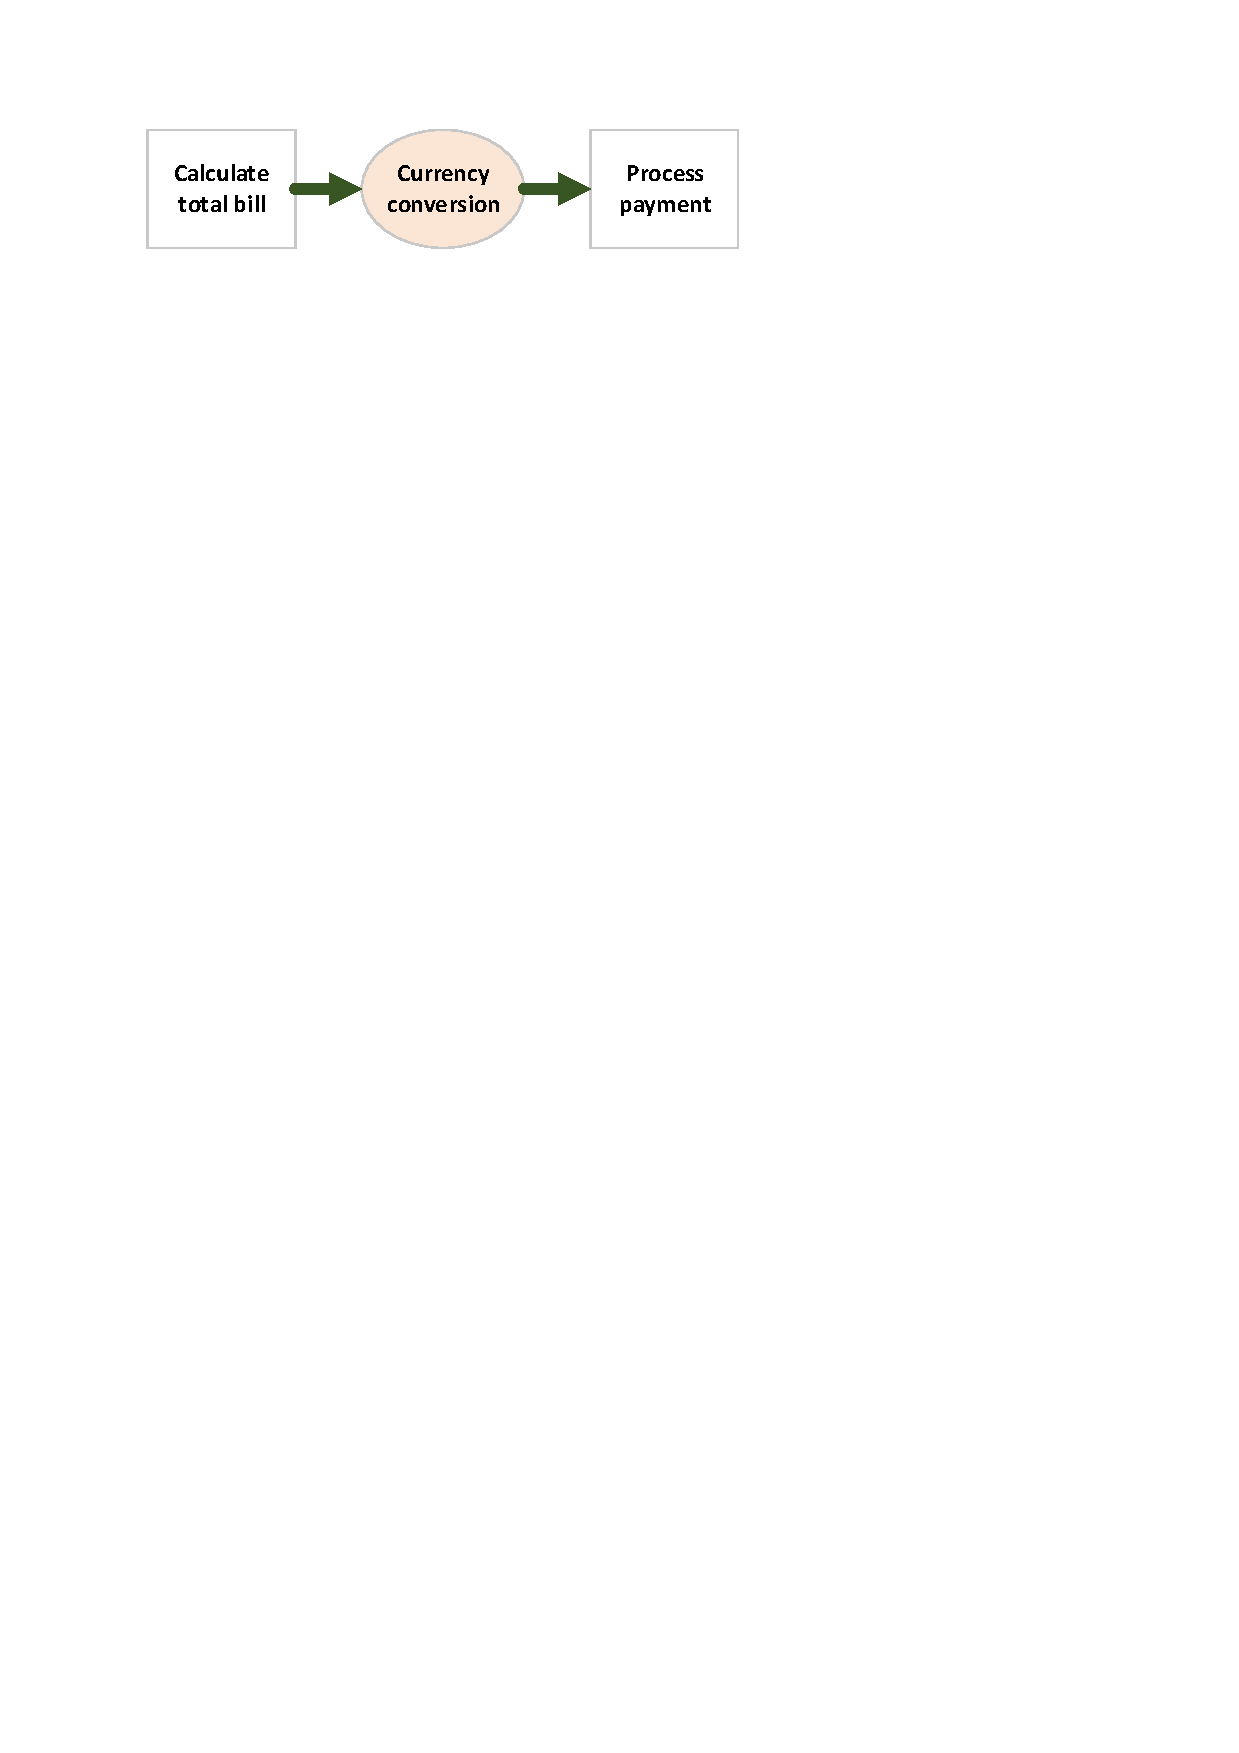
\includegraphics[width=7cm]{currency_example.pdf}}
\vfill
\begin{block}{Web service}
A functionality module that provides operations accessible over the network via a standard communication protocol.
\end{block}
\end{frame}

\note{
\begin{itemize}
 \item As the web becomes more and more pervasive, so does the concept of Service-Oriented Architecture.
 \item The idea in SOA is to organise business processes and data into independent modules which can then be reused in applicactions as needed.
 \item  For example, an e-commerce website may need to perform currency conversion depending on the location of its current customer, and so it uses an already existing currency conversion module.
 \item The basic components in SOA are services, which are functionality modules accessible over the network. In this example, currency conversion is a Web service.
\end{itemize}
}

%------------------------------------------------

\begin{frame}
\frametitle{Web Service Composition}
The combination of Web services to achieve a more complex task. Fully automated scenario:
\vfill
\centerline{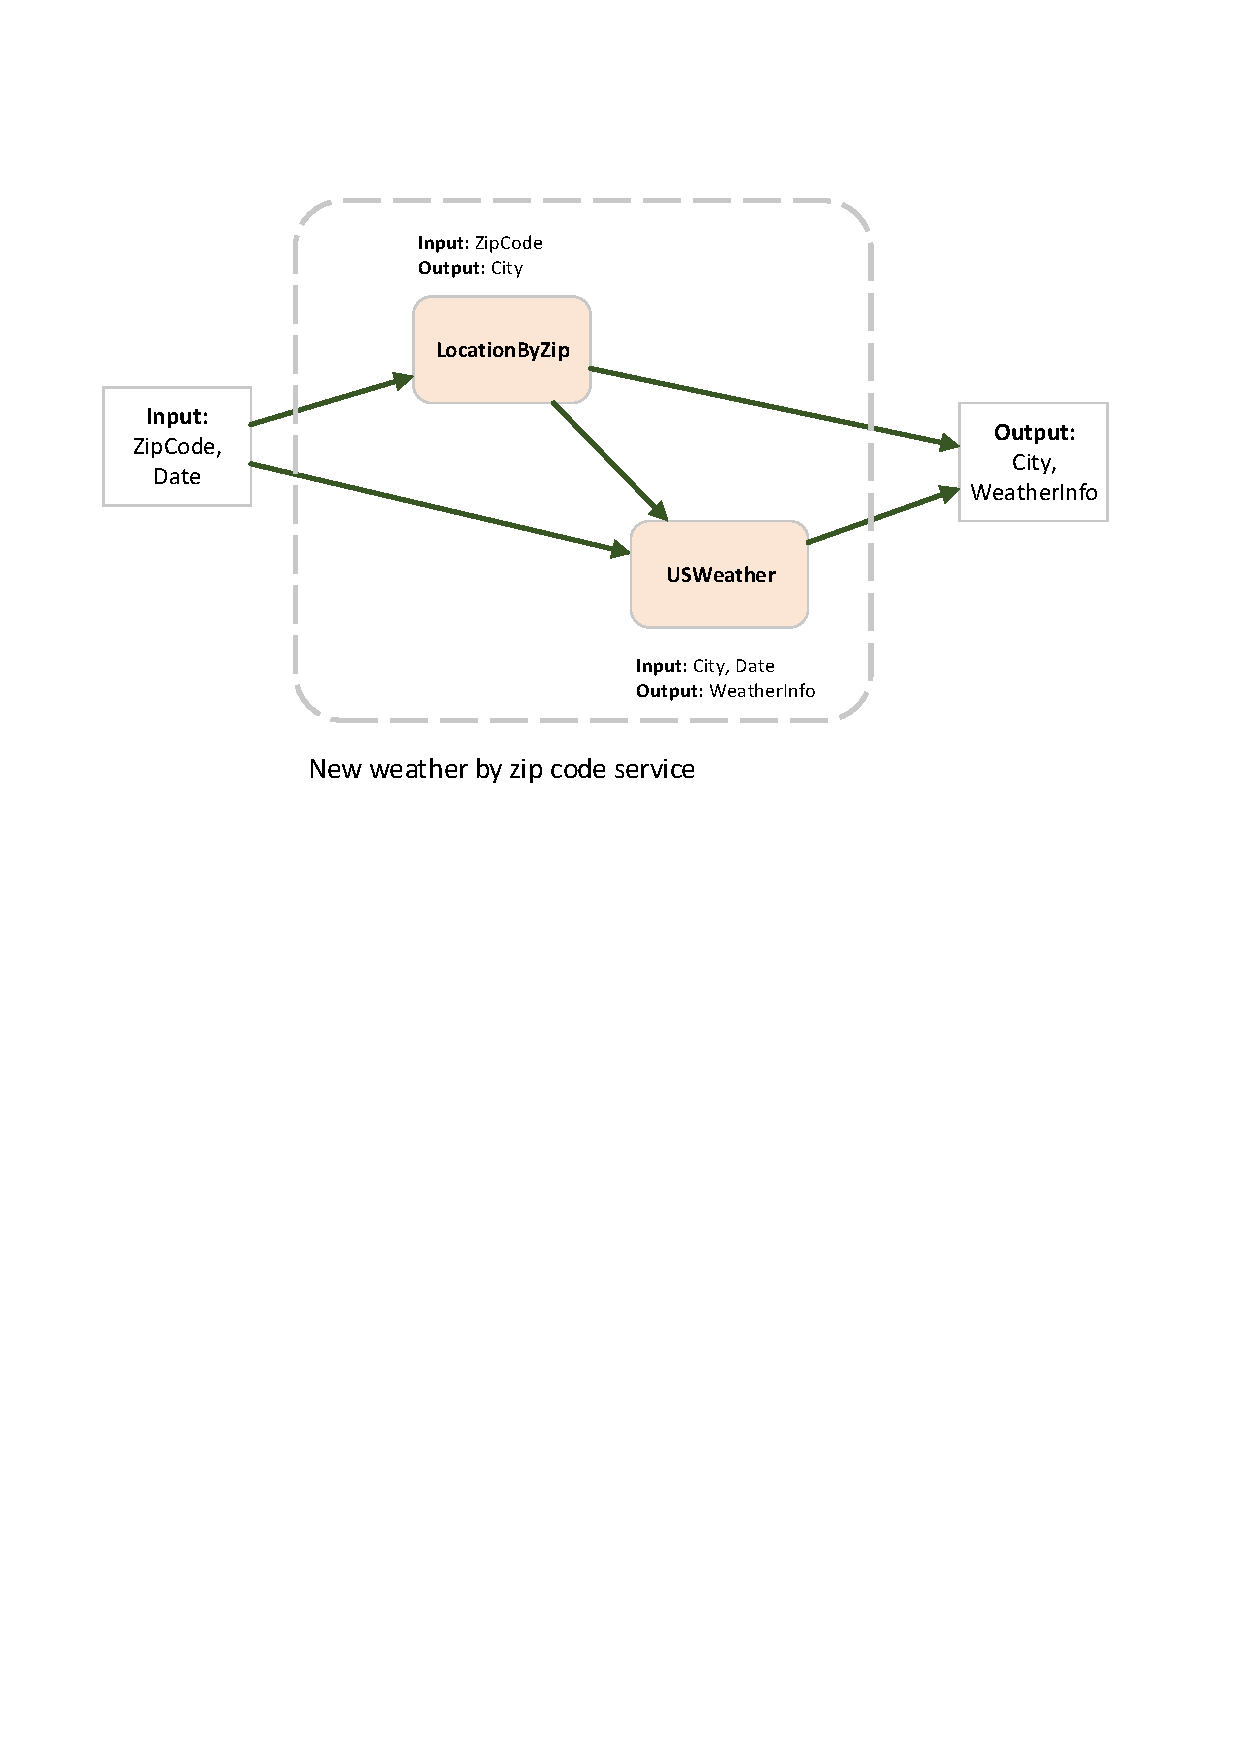
\includegraphics[width=10cm]{fully_automated_example.pdf}}
\end{frame}

\note{
\begin{itemize}
 \item The combination of multiple modular Web services in order to achieve a single, more complex task is known as Web service composition.
 \item Developing a system capable of creating such compositions in a fully automated manner is one of the holy grails of the field.
 \item With full automation, new services can be created simply by specifying the inputs the new service should require and the outputs it should produce, and the resulting composition is treated as a black box.
 \item For example, imagine we need to create a service that provides the weather forecast of a location based on its ZIP code. An automated composition system could identify and connect two different services, one that identifies a city based on a ZIP code and another that uses the city and date information to produce the forecast.
\end{itemize}
}

%------------------------------------------------

\begin{frame}
 \frametitle{A Composition Example with Branching}
 \begin{columns}
 \column{0.6\textwidth}
 \centerline{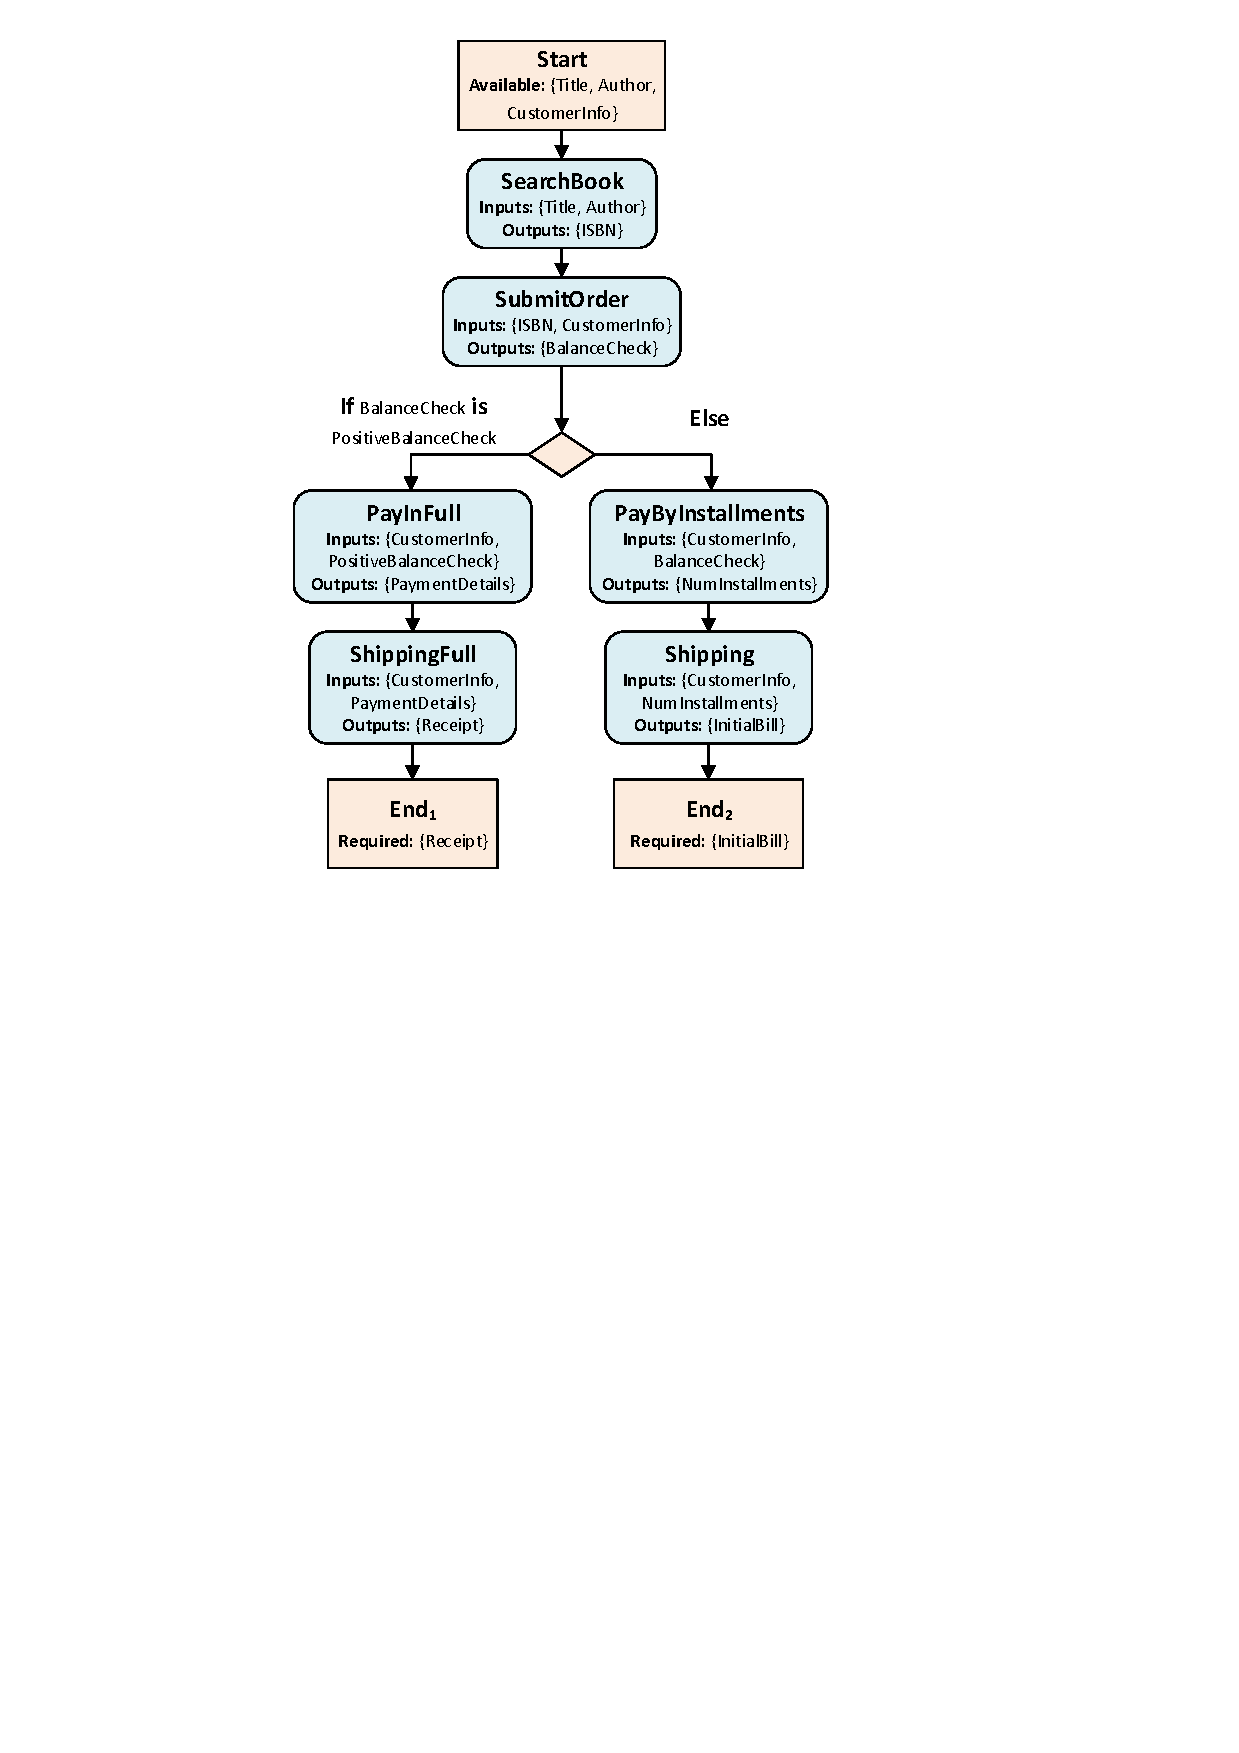
\includegraphics[width=4.5cm]{motivation.pdf}}
 
 \column{0.4\textwidth}
 Certain compositions require alternative paths according to runtime values.
 \bigskip
 
 \textbf{Example:} Depending on balance, pay in full or pay in installments.
 \end{columns}
\end{frame}

\note{
\begin{itemize}
 \item In certain cases, we might need alternative paths in a composition, depending on the runtime values produced.
 \item For example, in the case of a service that models the purchase of a book, the customer might pay for the book in full or in installments, depending on their current balance.
 \item So, once the balance is check, one of two different branches may be executed, leading to different outputs.
\end{itemize}

}

%------------------------------------------------

\begin{frame}
\frametitle{Composition Dimensions}
\begin{enumerate}
\item \textbf{Functional correctness:} Service inputs and outputs must be properly linked (e.g. \textcolor{blue}{$FourDigitNumber \rightarrow ZipCode$}, but not \textcolor{blue}{$FourDigitNumber \rightarrow City$}).
\vfill
\item \textbf{Conditional constraints:} Condition leading to multiple possible execution paths (e.g. if \textcolor{blue}{$City$} is a \textcolor{blue}{$NewZealandCity$}, produce \textcolor{blue}{$WindForecast$} instead of \textcolor{blue}{$GeneralForecast$}).
\vfill
\item \textbf{Quality of Service (QoS):} The overall quality of the composition (e.g. \textcolor{blue}{lowest execution time}, \textcolor{blue}{lowest cost}).
\end{enumerate}
\end{frame}

\note{
\begin{itemize}
 \item As we can see, the complexity of Web service composition lies in the number of different dimensions it must consider at the same time.
 \item In the first dimension, we must ensure that services have their inputs and outputs properly linked. For example, a service that produces a four-digit number should be able to feed its output to the input of a service that accepts a zip code, however a four-digit number should not be accepted as a city name.
 \item In the second dimension, we must consider conditions that lead to different execution paths. For example, if a city is located in New Zealand, we would like a wind-only forecast as opposed to a general one.
 \item In the third dimension, we must produce compositions with the best possible quality attributes. For example, we would like it to have the lowest possible execution time as well as the lowest possible financial cost.
\end{itemize}

}

%------------------------------------------------

\begin{frame}
\frametitle{Existing Approaches}
{
\setbeamercolor{block title}{bg=red!40, fg=black}
\begin{block}{\textbf{AI Planning}}
Build a solution service by service.\\
Dimensions: \textit{Functional correctness, conditional constraints.}
\end{block}
}

\vfill
{
\setbeamercolor{block title}{bg=green!40, fg=black}
\begin{block}{\textbf{Evolutionary Computation (EC)}}
Improve population of solutions over multiple generations.\\
Dimensions: \textit{Functional correctness, QoS.}
\end{block}
}

\vfill
{
\setbeamercolor{block title}{bg=cyan!40, fg=black}
\begin{block}{\textbf{Hybrid Approaches}}
Combine AI planning and EC ideas.\\
Dimensions: \textit{Functional correctness, QoS.}
\end{block}
}
\end{frame}

\note{
\begin{itemize}
 \item Several techniques have been proposed to address the composition problem, however these approaches only account for at most two dimensions at once.
 \item In AI planning, a solution is built step by step, in each step adding a service and verifying the overall state of the composition. This approach typically verifies functional correctness and conditional constraints, but not the overall QoS.
 \item In evolutionary computation, a population of solutions is created and improved over multiple generations. This approach typically verifies functional correctness and optimises the overall QoS, but does not address conditional constraints.
 \item Hybrid approaches combine elements of AI planning and EC, making it easier to check the functional correctness and at the same time optimise the overall QoS. However, this approach also fails to address conditional constraints.
\end{itemize}
}

%------------------------------------------------

\begin{frame}
\frametitle{Goal}
To propose a Genetic Programming (GP) composition approach that simultaneously considers all dimensions.
\vfill

\begin{columns}[c]
\column{0.3\textwidth}
\begin{enumerate}
 \item Trees preserve functional correctness.
 \vfill
 \item Conditions encoded in trees.
 \vfill
 \item Optimisation performed on QoS.
\end{enumerate}

\column{0.5\textwidth}
\centerline{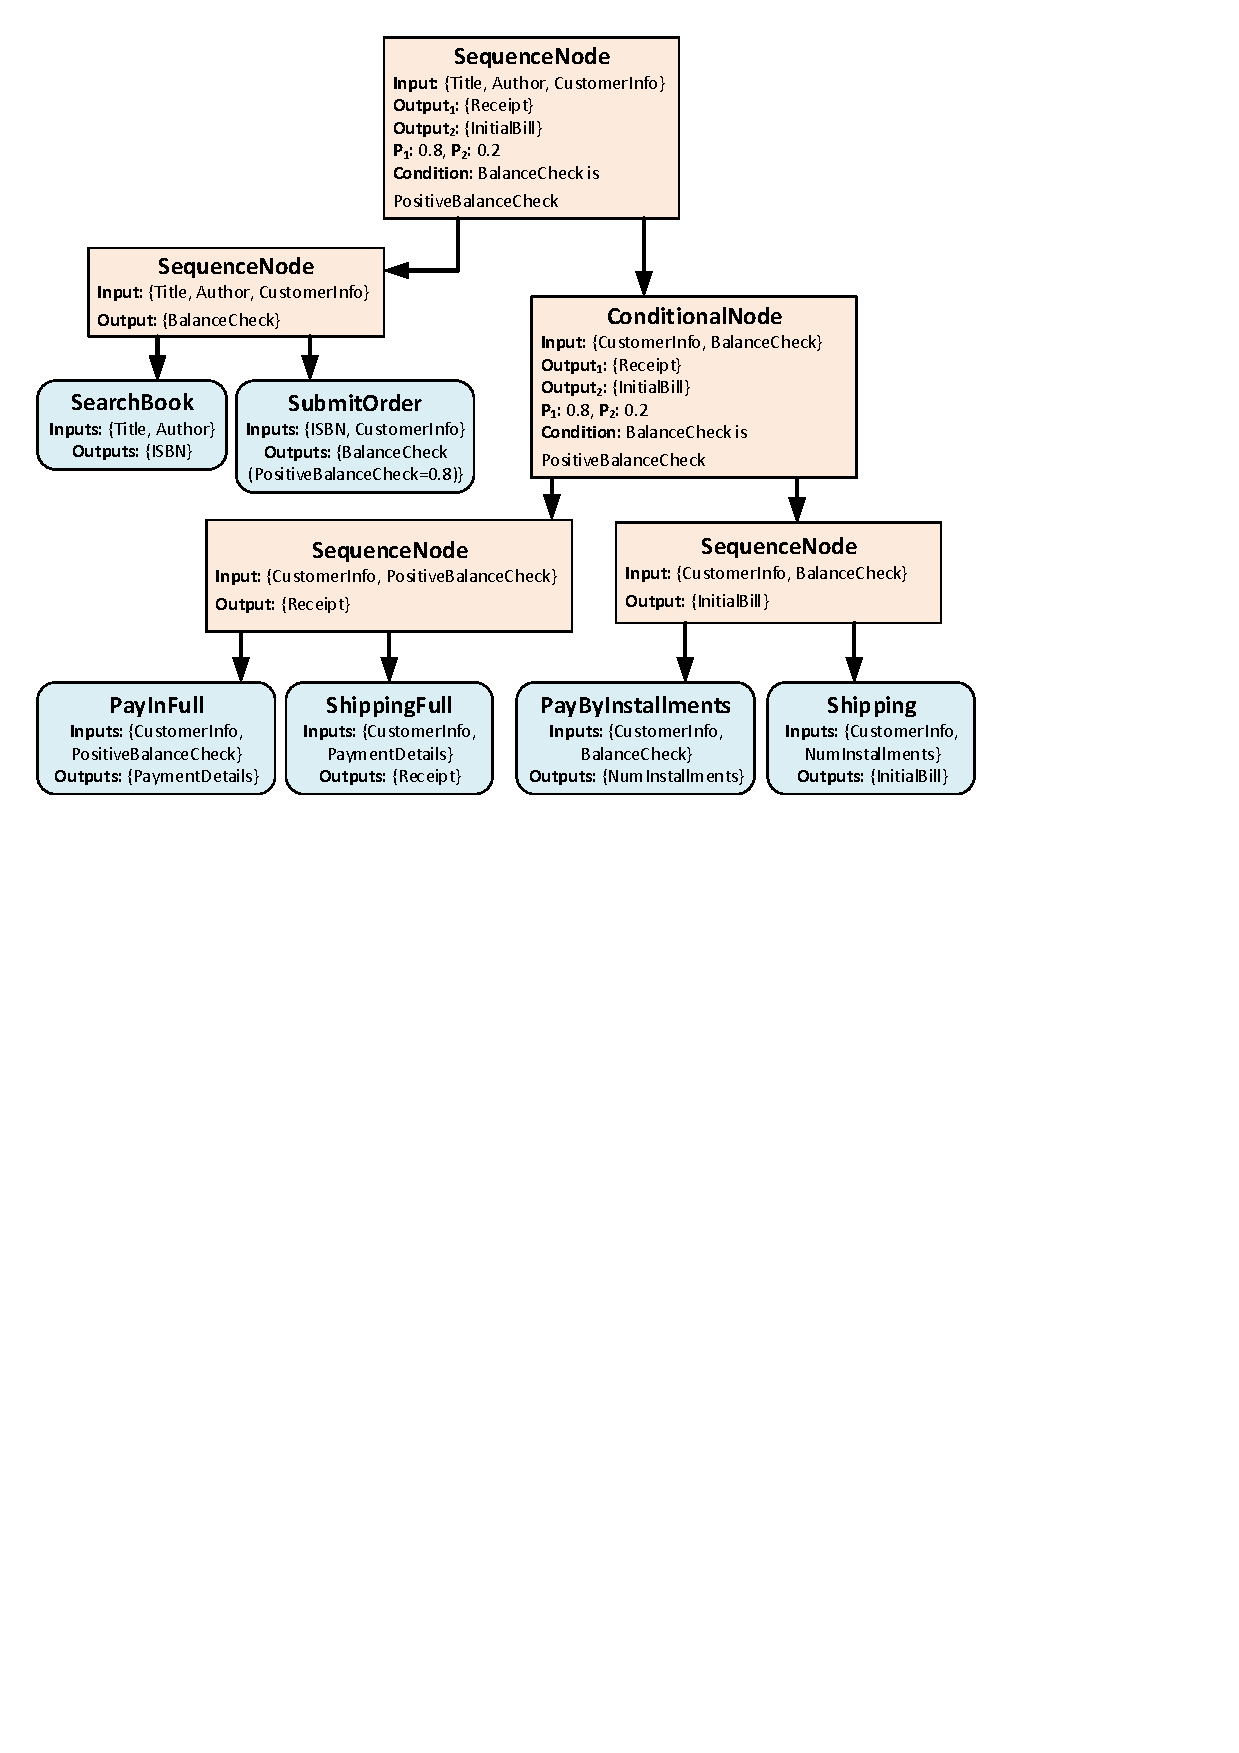
\includegraphics[width=6cm]{tree.pdf}}
\end{columns}

\end{frame}

\note{
\begin{itemize}
 \item Given these limitations, the objective of the approach proposed in this paper is to address these three dimensions simultaneously by using genetic programming.
 \item The functional correctness dimension is addressed by restricting the way in which services are linked to each other in each solution tree.
 \item Conditional constraints are addressed by including a conditional nodes as possible nodes in the tree representation.
 \item The Quality of Service dimension is addressed by using a fitness function that optimises solutions on quality attributes.
 \item Let's understand these in more detail.
\end{itemize}

}

%------------------------------------------------
\section{GP Approach}
\subsection{}
%------------------------------------------------

\begin{frame}
 \frametitle{Candidate Representation}
 \begin{columns}
 \column{0.6\textwidth}
 \centerline{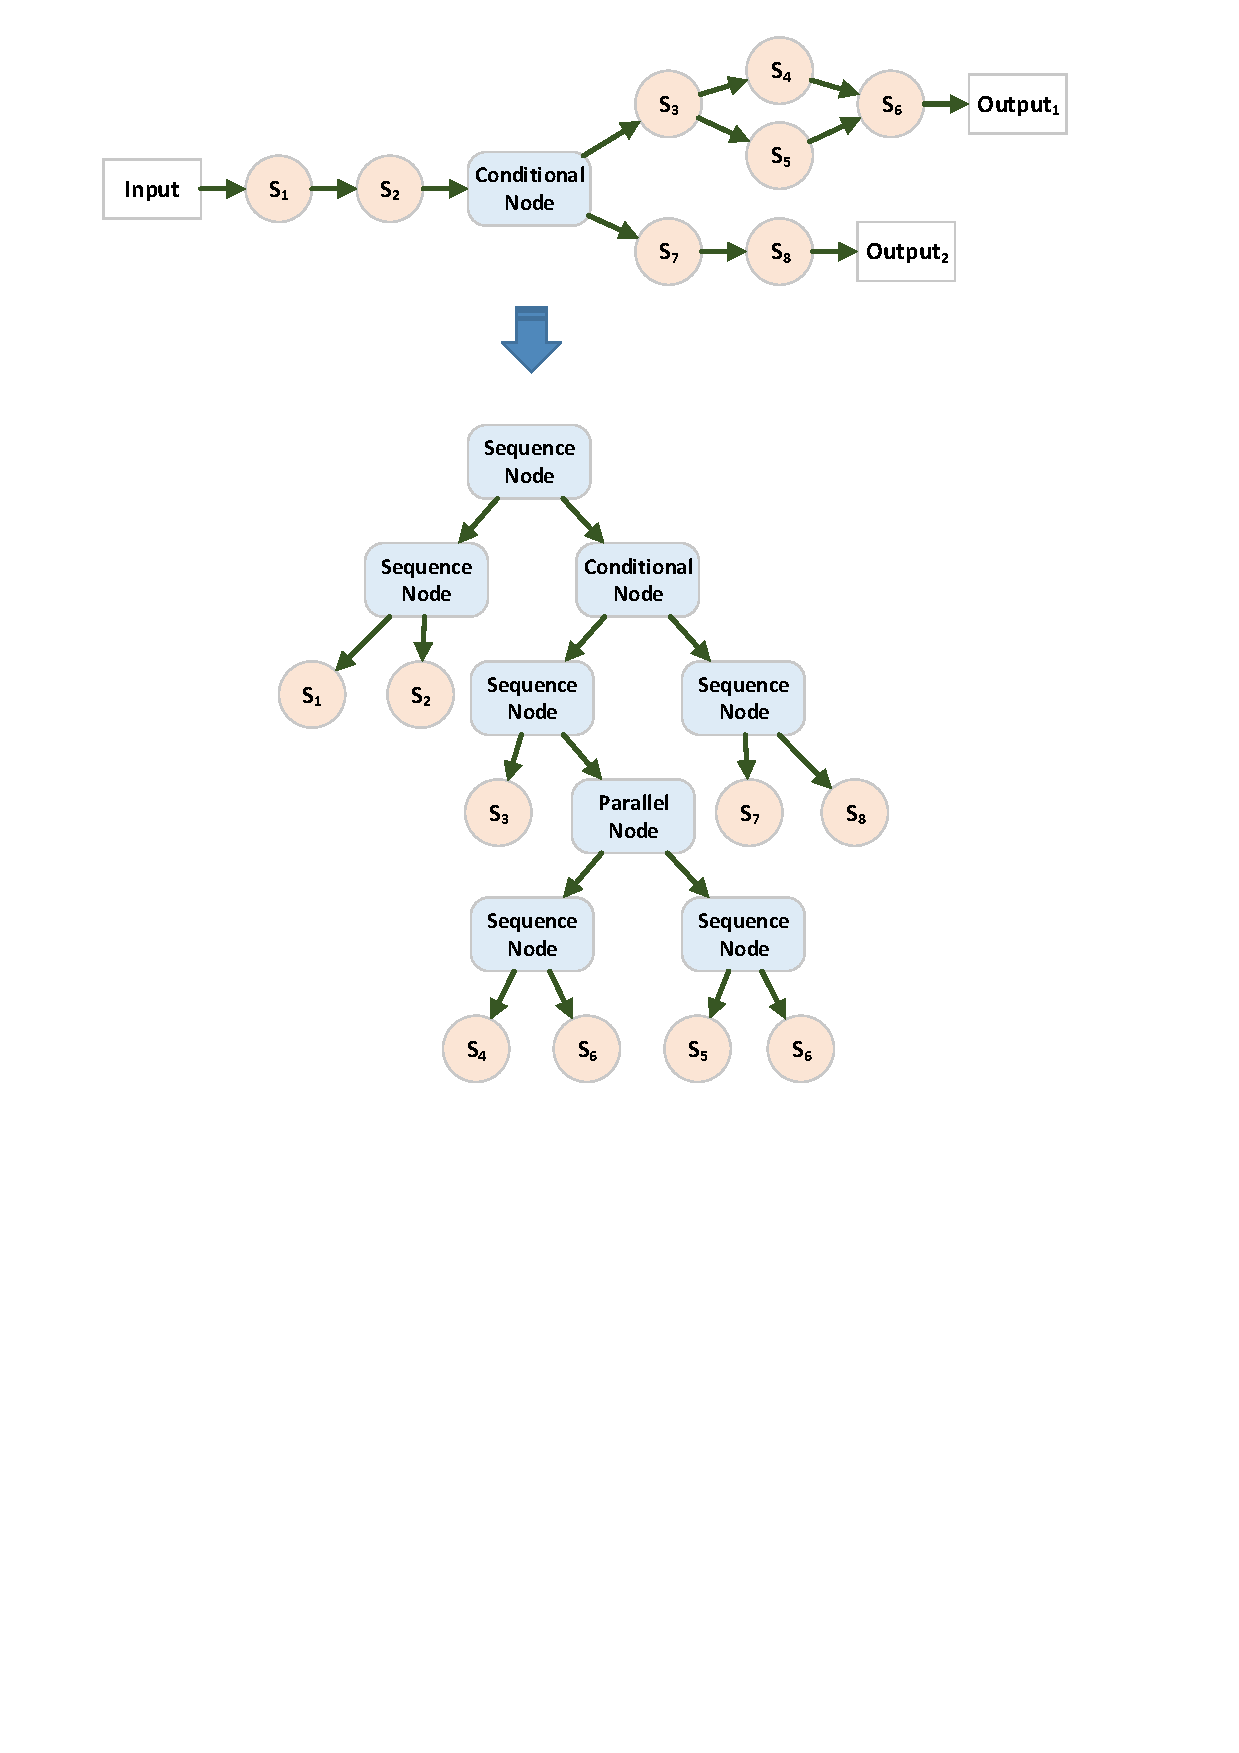
\includegraphics[width=6.5cm]{representation.pdf}}
 
 \column{0.4\textwidth}
 \begin{itemize}
  \item Tree equivalent to graph composition.
  \medskip
  \item  Parallel, sequential, and conditional represented as non-terminal nodes.
  \medskip
  \item Candidate services as terminal nodes.
 \end{itemize}

 \end{columns}
\end{frame}

\note{
	\begin{itemize}
	\item Web service compositions can be intuitively represented as directed acyclic graphs, as shown by the first structure. We can see that parallel and sequential configurations are encoded by the edges, and conditional constraints by special nodes.
	\item However, a tree representation is required for GP. Therefore, in our approach parallel, sequential, and conditional configurations are all represented as non-terminal nodes of the tree, while candidate atomic services are the terminal nodes.
	\item The tree structure shown here is equivalent to the composition shown in graph form.
	\end{itemize}
}

%------------------------------------------------

\begin{frame}
\frametitle{Population Initialisation}
An algorithm is used to create a candidate in graph format, and then translate it into a tree representation.

\vfill

\begin{columns}[c]
\column{7cm}
\hspace{1cm}
%\centerline{
\fbox{
\scalebox{.40}{
\begin{algorithm*}[H]
 \setlength\hsize{0.9\linewidth}
 \SetKwInOut{Input}{Input}\SetKwInOut{Output}{Output}
 \SetKwFunction{createGraph}{createGraph}\SetKwFunction{toTree}{toTree}
 \LinesNumbered
 \SetNlSty{}{}{:}
 \Input{$I$, $O_1$, $O_2$, $C$, $P$}
 \Output{candidate tree $T$}
 \eIf{$O_2 \neq \emptyset$}{
  $G_1 \leftarrow \createGraph(I \cup C.if, O_1)$\;
  $G_2 \leftarrow \createGraph(I \cup C.else, O_2)$\;
  $T_1 \leftarrow \toTree(G_1.input)$\;
  $T_2 \leftarrow \toTree(G_2.input)$\;
  $T_3 \leftarrow$ new $ConditionalNode$($C$)\;
  $T_3.leftChild \leftarrow T_1$\;
  $T_3.rightChild \leftarrow T_2$\;
  \eIf{$C \sqsubseteq I$}{
    $T_3.prob \leftarrow P$\;
    \KwRet $T_3$\;
  }{
    $G_4 \leftarrow \createGraph(I, C.else)$\;
    $T_4 \leftarrow \toTree(G_4.input)$\;
    $T_3.prob \leftarrow T_4.final.P$\;
    $T \leftarrow$ new $SequenceNode$()\;
    $T.leftChild \leftarrow T_4$\;
    $T.rightChild \leftarrow T_3$\;
    \KwRet $T$\;
  }
 }{
  $G \leftarrow \createGraph(I, O_1)$\;
  $T \leftarrow \toTree(G.input)$\;
  \KwRet $T$\;
 }
% \vspace{2mm}
% \caption{\footnotesize Generating a new candidate tree or a mutated subtree.}
%\label{generation}
\end{algorithm*}
}}%}

\column{4cm}
\hspace{-2cm}
\centerline{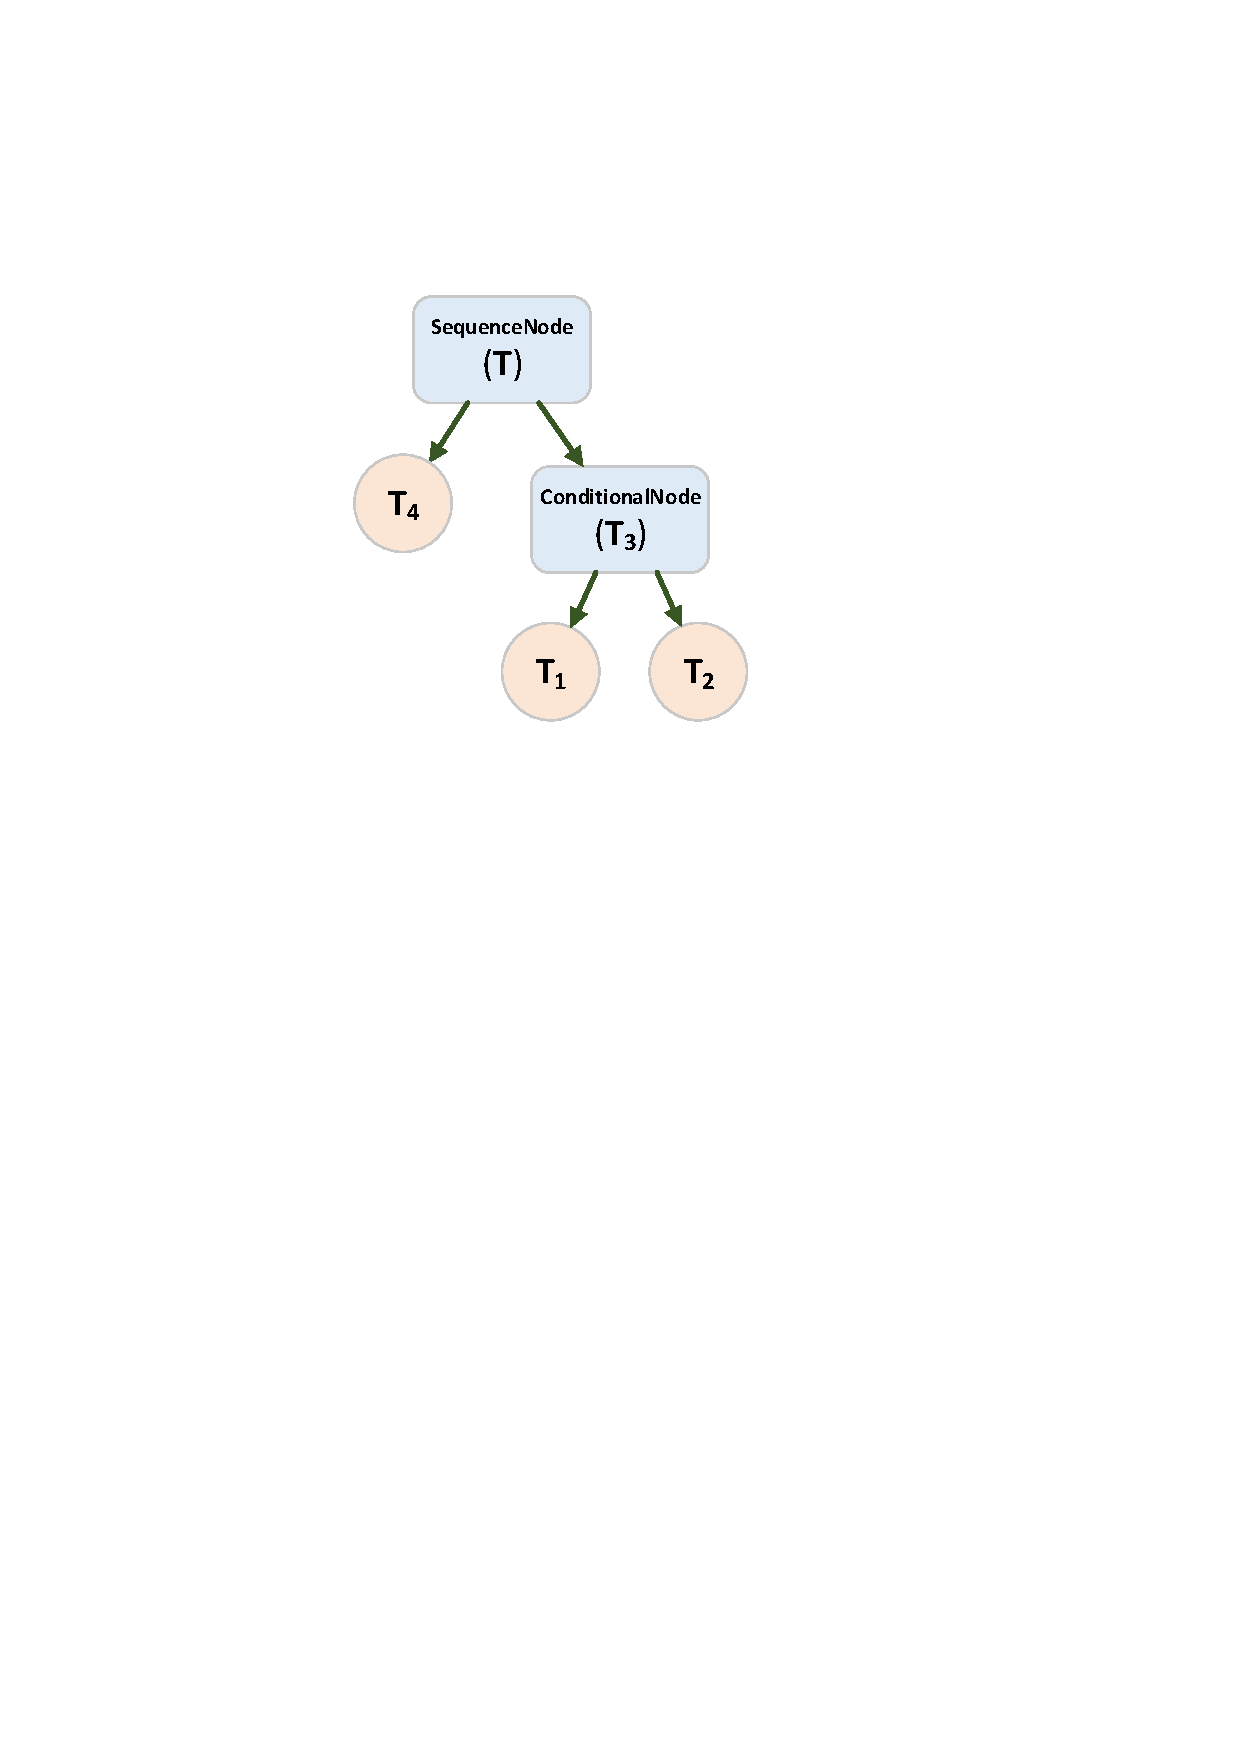
\includegraphics[width=4cm]{algorithm_tree.pdf}}
\end{columns}
\end{frame}

\note{
	\begin{itemize}
	\item In order to create candidates with correct input-output connections between services, we employ an initialisation algorithm that creates compositions in graph form and then translates them into tree form.
	\item The basic idea of this algorithm is to build each part of the tree separately, and then assemble the parts into a candidate. Each part is built ensuring that the connections are correct. We begin by building the parts that go from the conditional node to the overall outputs ($T_1$ and $T_2$), and both possibilities are built. Then we move on to the part that leads to the condition from the overall inputs ($T_4$). These are connected to a sequence and a conditional node.
	\item For simplicity, in this work we assume that each composition has only one conditional node, so its position is always the same in the tree.
	\end{itemize}
}

%------------------------------------------------

\begin{frame}
\frametitle{Mutation and Crossover}
\begin{columns}[c]
\column{0.4\textwidth}
\minipage[c][0.7\textheight][s]{\columnwidth}
\textbf{Mutation:} Selects random node and replaces it with equivalent subtree.
\vfill
\centerline{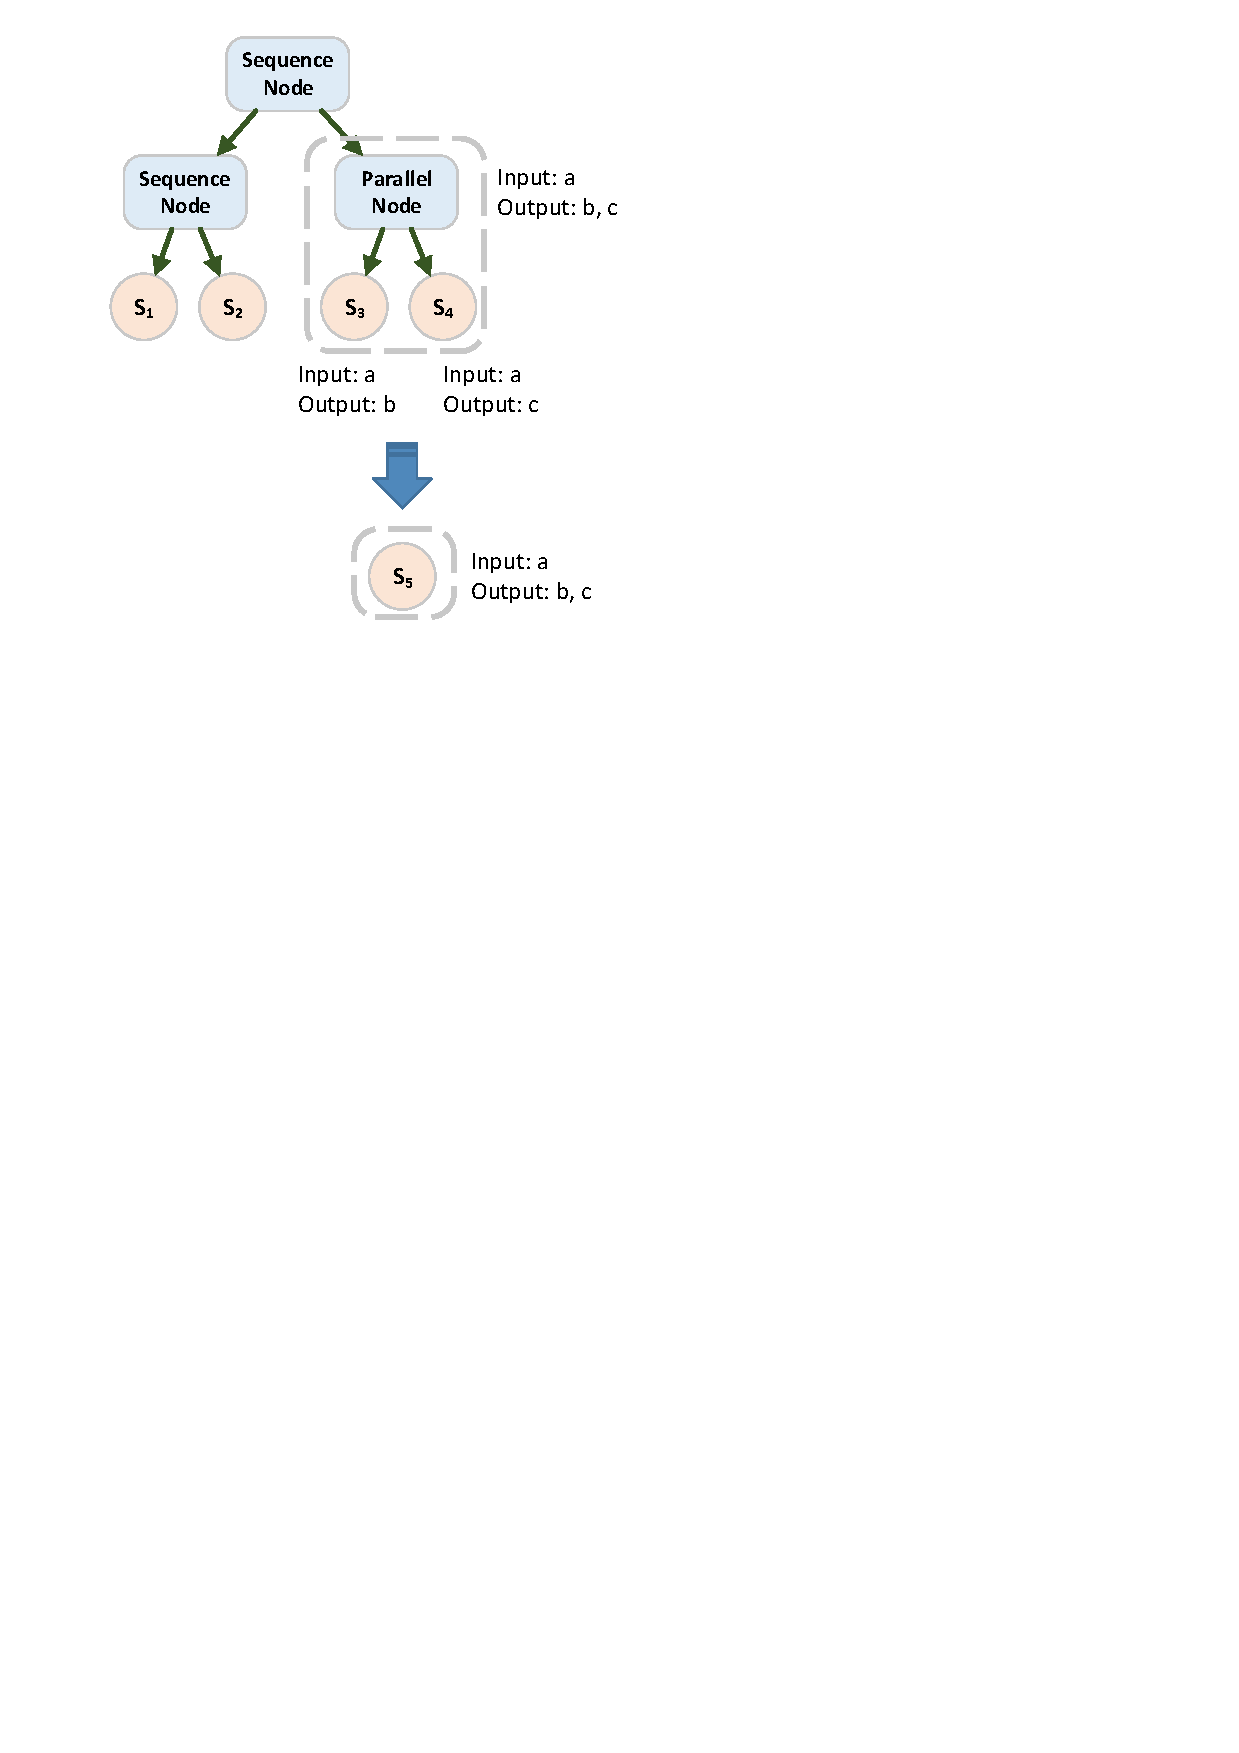
\includegraphics[width=4cm]{mutation.pdf}}
\endminipage

\column{0.4\textwidth}
\minipage[c][0.7\textheight][s]{\columnwidth}
\textbf{Crossover:} Swaps any two equivalent terminal nodes.

{
\smallskipamount=0.5cm
\smallskip
}
\centerline{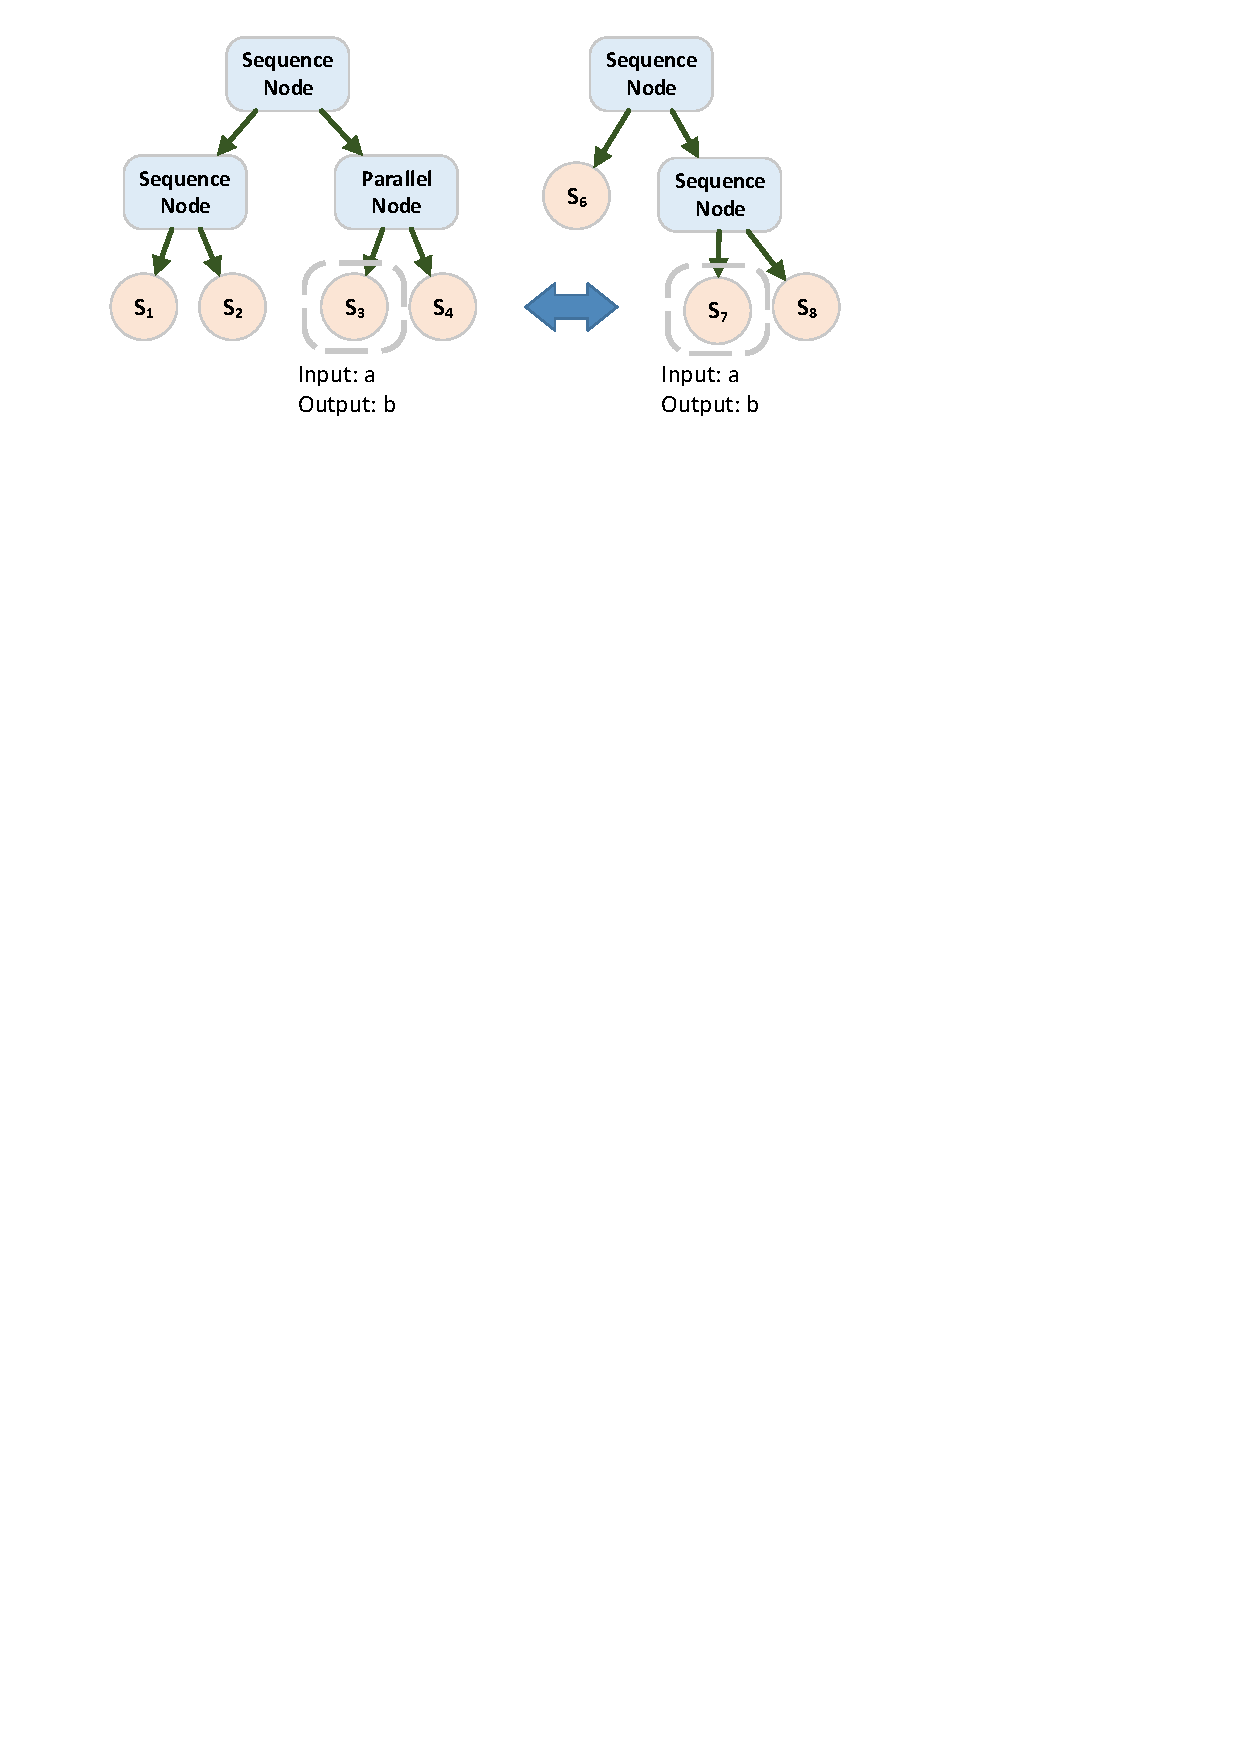
\includegraphics[width=6cm]{crossover.pdf}}
\endminipage
\end{columns}
\end{frame}

\note{
	\begin{itemize}
		\item During the evolution process, the custom operators used are mutation and crossover. Both of these operators maintain the functional correctness of candidates, that is, they ensure that input-output connections still make sense.
		\item The mutation operator randomly selects a node in the tree, removes that subtree and replaces it with a newly generated subtree. The new subtree may have a different structure than the old one, but it is functionally equivalent to it, i.e. produces the same output given the same input. New subtrees are generated using the initialisation algorithm.
		\item The crossover operator finds any functionally equivalent terminal nodes in two candidate trees and swaps them. We chose this crossover operation because it models the process of Web service selection, where the best service is chosen among a group of functionally equivalent candidates.
	\end{itemize}
}

%------------------------------------------------

\begin{frame}
\frametitle{Fitness Function}
Measures the overall quality of a composition candidate (minimising).

\vfill

\centerline{
$fitness_i = w_1(1 - A_i) + w_2(1 - R_i) + w_3T_i + w_4C_i$
}
\bigskip

\centerline{
\noindent where $\sum_{i=1}^{4} w_i = 1$
}


\vfill
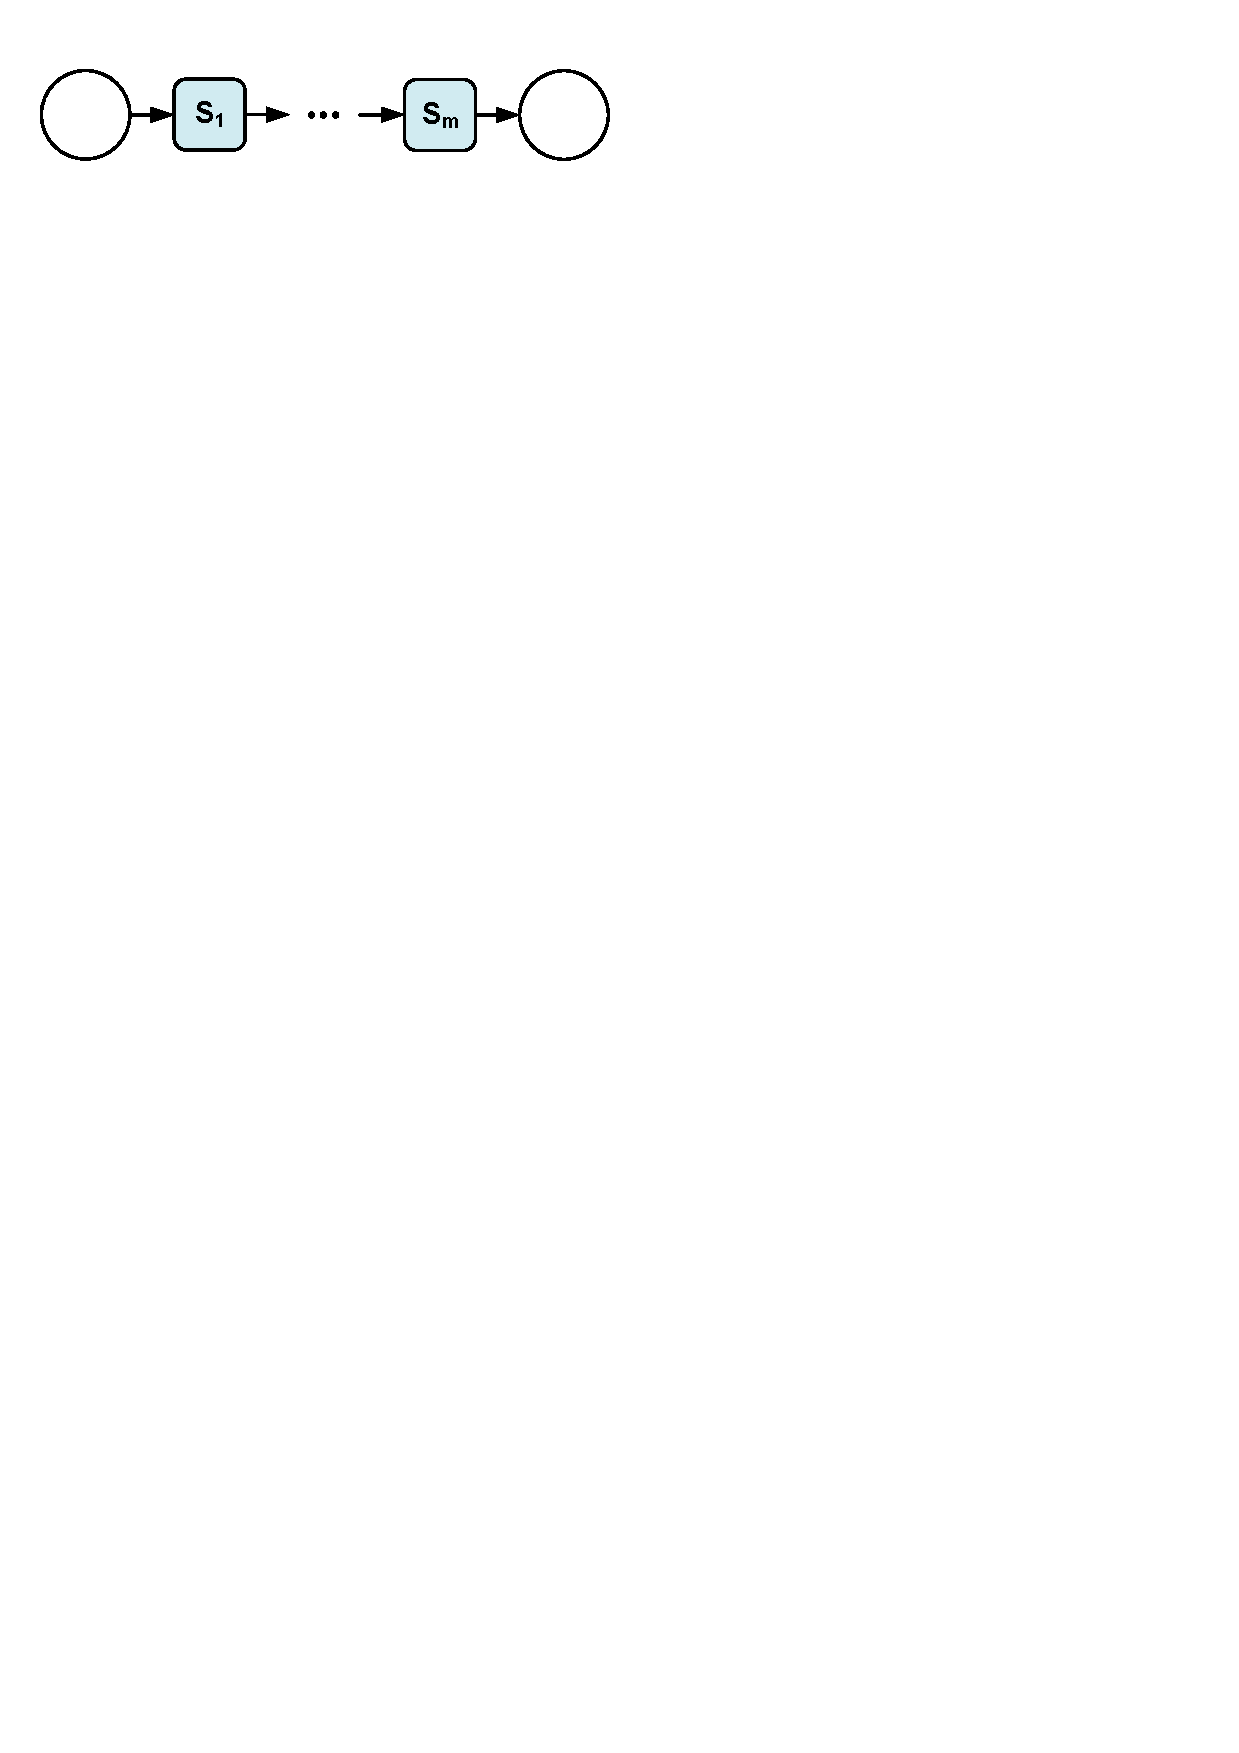
\includegraphics[width=4cm]{sequence.pdf}
\hfill
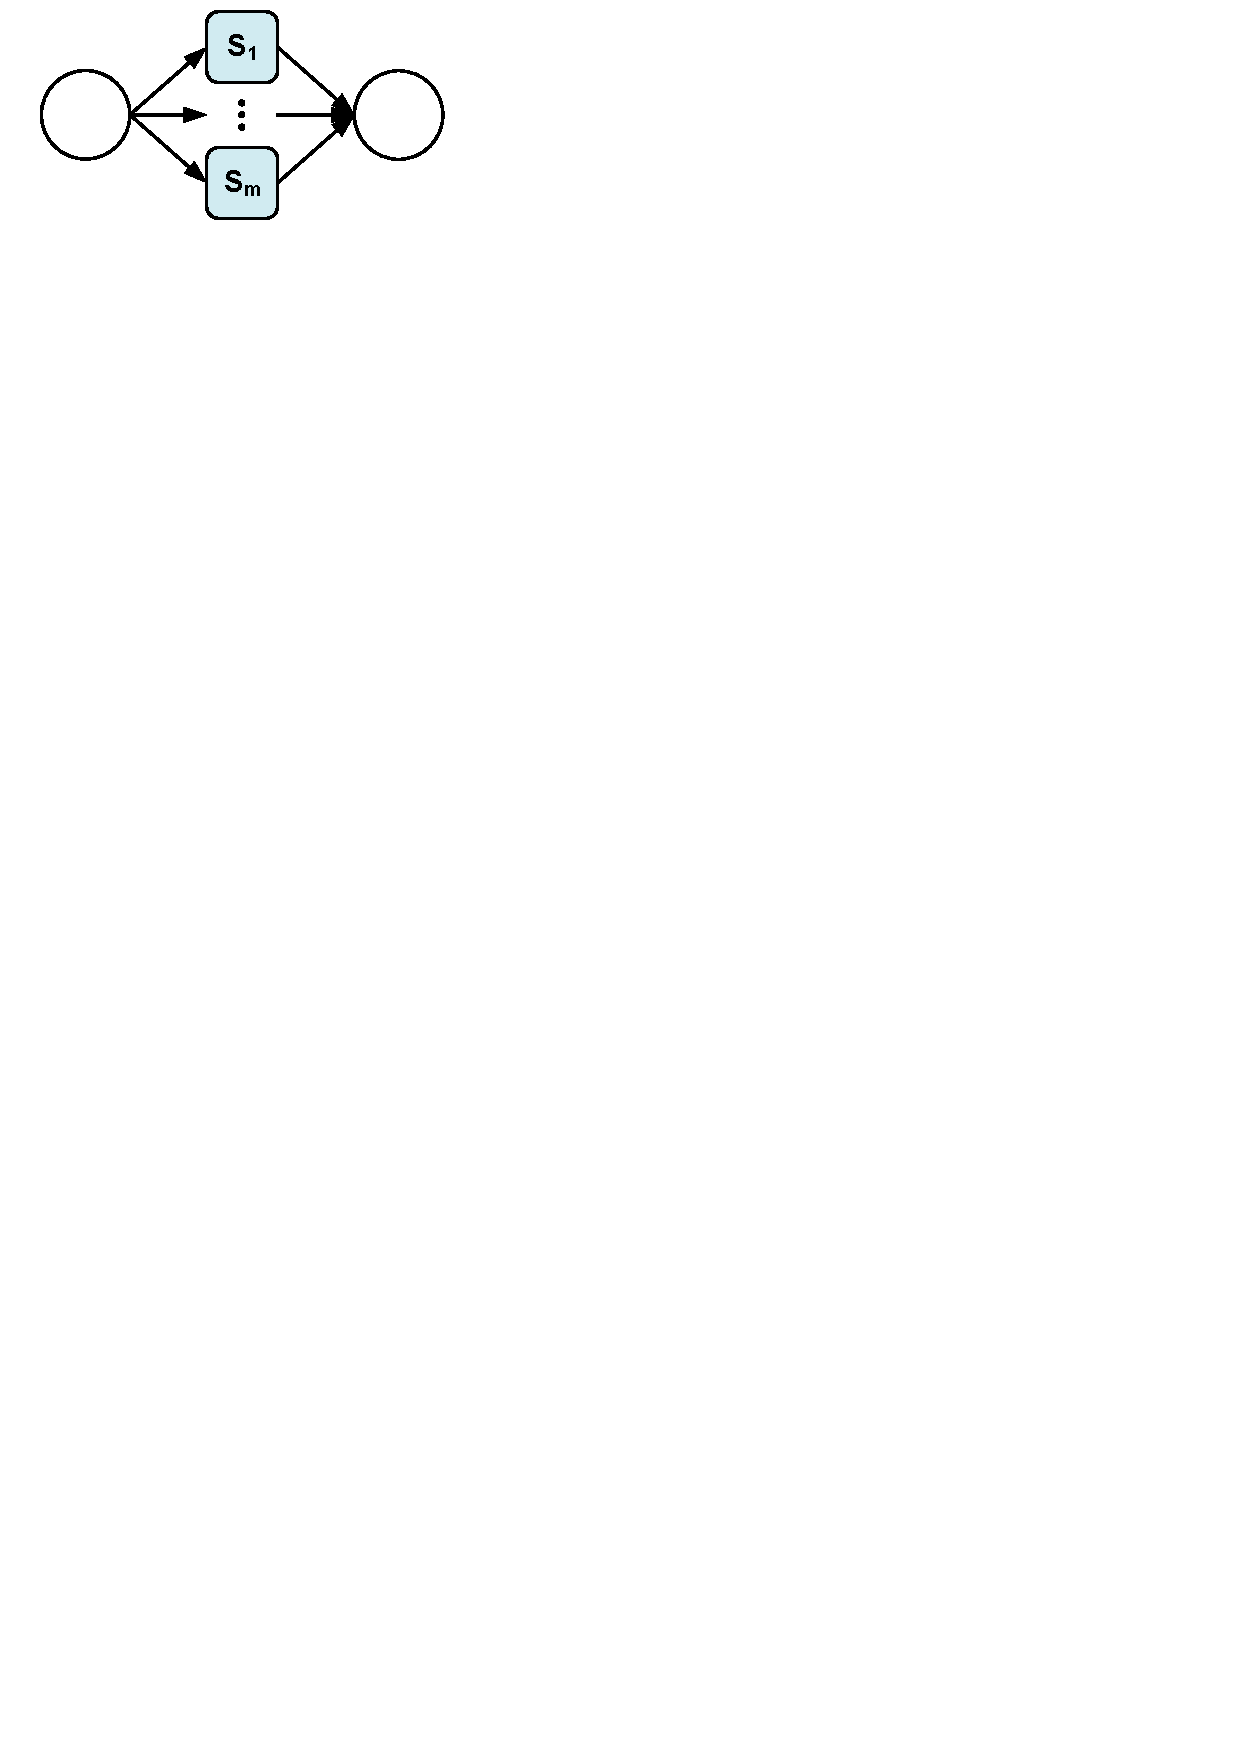
\includegraphics[width=2.7cm]{parallel.pdf}
\hfill
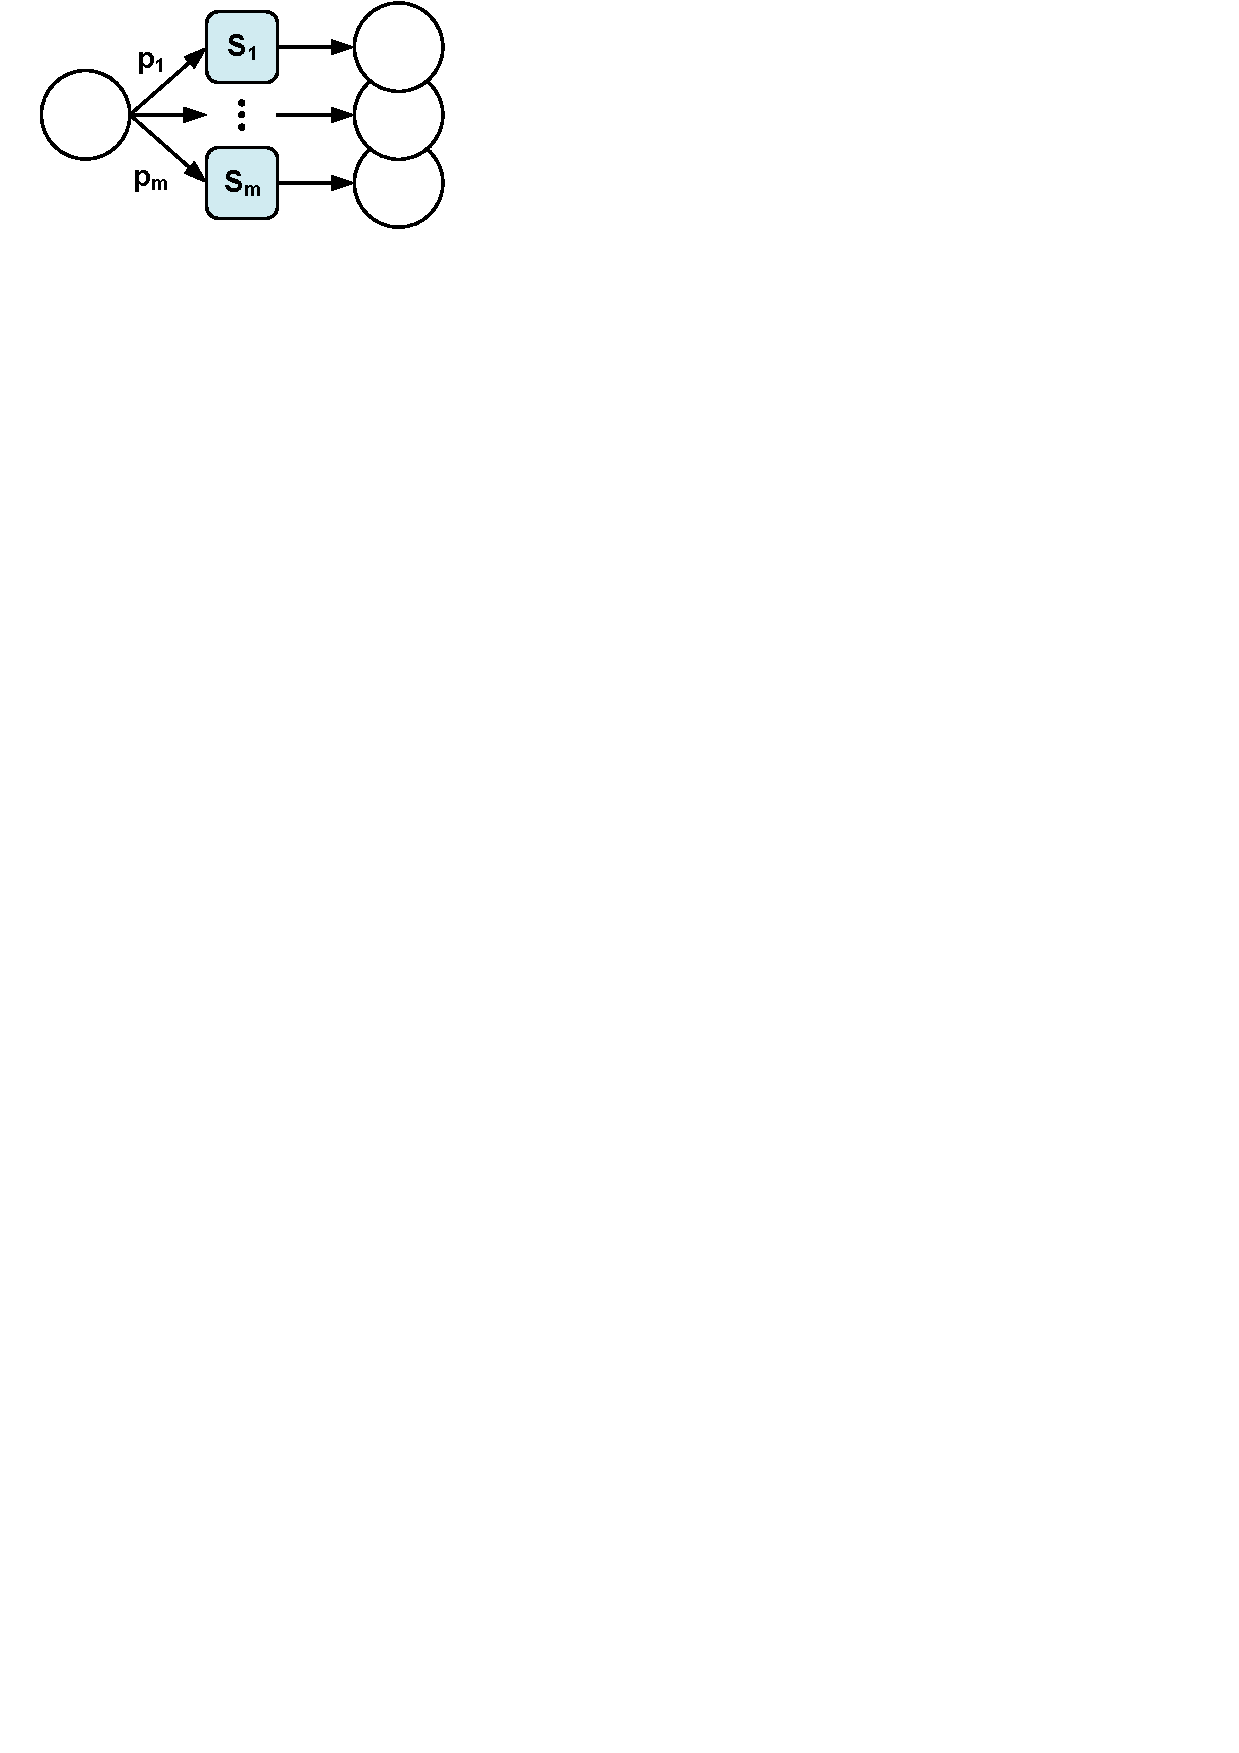
\includegraphics[width=2.7cm]{conditional.pdf}

\end{frame}

\note{
\begin{itemize}
 \item The fitness function is used to optimise the composition candidates according to their overall quality of service attributes. The values produced range from 0, in the best possible case, to 1, in the worst possible.
 \item These attributes are combined into a single value by using a weighted sum, where the weights add up to 1. The individual QoS values are also normalised to remain between 0 and 1.
 \item The different overall quality attributes are calculated differently depending on the constructs of the composition. For example, the execution time is the sum of individual service times in a sequential construct; it is the longest individual time in a parallel construct; it is a weighted sum of individual times, where the weights are probabilities, in a branching construct.
\end{itemize}

}

%------------------------------------------------
\section{Experiments}
\subsection{}
%------------------------------------------------

\begin{frame}
\frametitle{Experiments}
\begin{itemize}
 \item Lack of datasets supporting composition with branching.
 \item Lack of comparable approaches that produce solutions with multiple output possibilities.
\end{itemize}

\setbeamercolor{postit}{fg=black,bg=orange!30}
\begin{beamercolorbox}[sep=1em]{postit}
\textbf{Decision:} Create datasets, execute for conditional compositions and also for each branch separately.
\end{beamercolorbox}

Parameters:
\begin{table}
\footnotesize
\def\arraystretch{1.5}
\begin{tabular}{|l|c|lcl}
\cline{1-4}
Independent runs      & 50  & \multicolumn{1}{l|}{Elitism candidates} & \multicolumn{1}{c|}{1}          &  \\ \cline{1-4}
Population size       & 20  & \multicolumn{1}{l|}{Tournament size}    & \multicolumn{1}{c|}{7}          &  \\ \cline{1-4}
Crossover probability & 0.9 & \multicolumn{1}{l|}{Fitness weights}    & \multicolumn{1}{c|}{0.25 (all)} &  \\ \cline{1-4}
Mutation probability  & 0.1 &                                         & \multicolumn{1}{l}{}            &  \\ \cline{1-2}
\end{tabular}
\end{table}

\end{frame}

\note{
\begin{itemize}
\item The performance of the proposed approach was evaluated through a set of experiments.
\item There were two big difficulties in conducting these experiments: firstly, there is a lack of existing datasets that support branching in the field; secondly, there are no other approaches that can be used for direct comparison (they have no branching and QoS optimisation simultaneously).
\item Having these problems in mind, our decision was to create our own datasets, and to run experiments both for conditional tasks with two branches and for the branches separately.
\item While definitive conclusions cannot be made by comparing the results with branching to those without branching, interesting patterns may nevertheless emerge.
\item The parameters shown here were used for testing.
\end{itemize}
}


%------------------------------------------------

\begin{frame}
\frametitle{Creation of Datasets}
Modified from WSC2008.

\begin{itemize}
 \item Can be extended to contain QoS.
 \item Provides ontology of input and output values.
\end{itemize}

\centerline{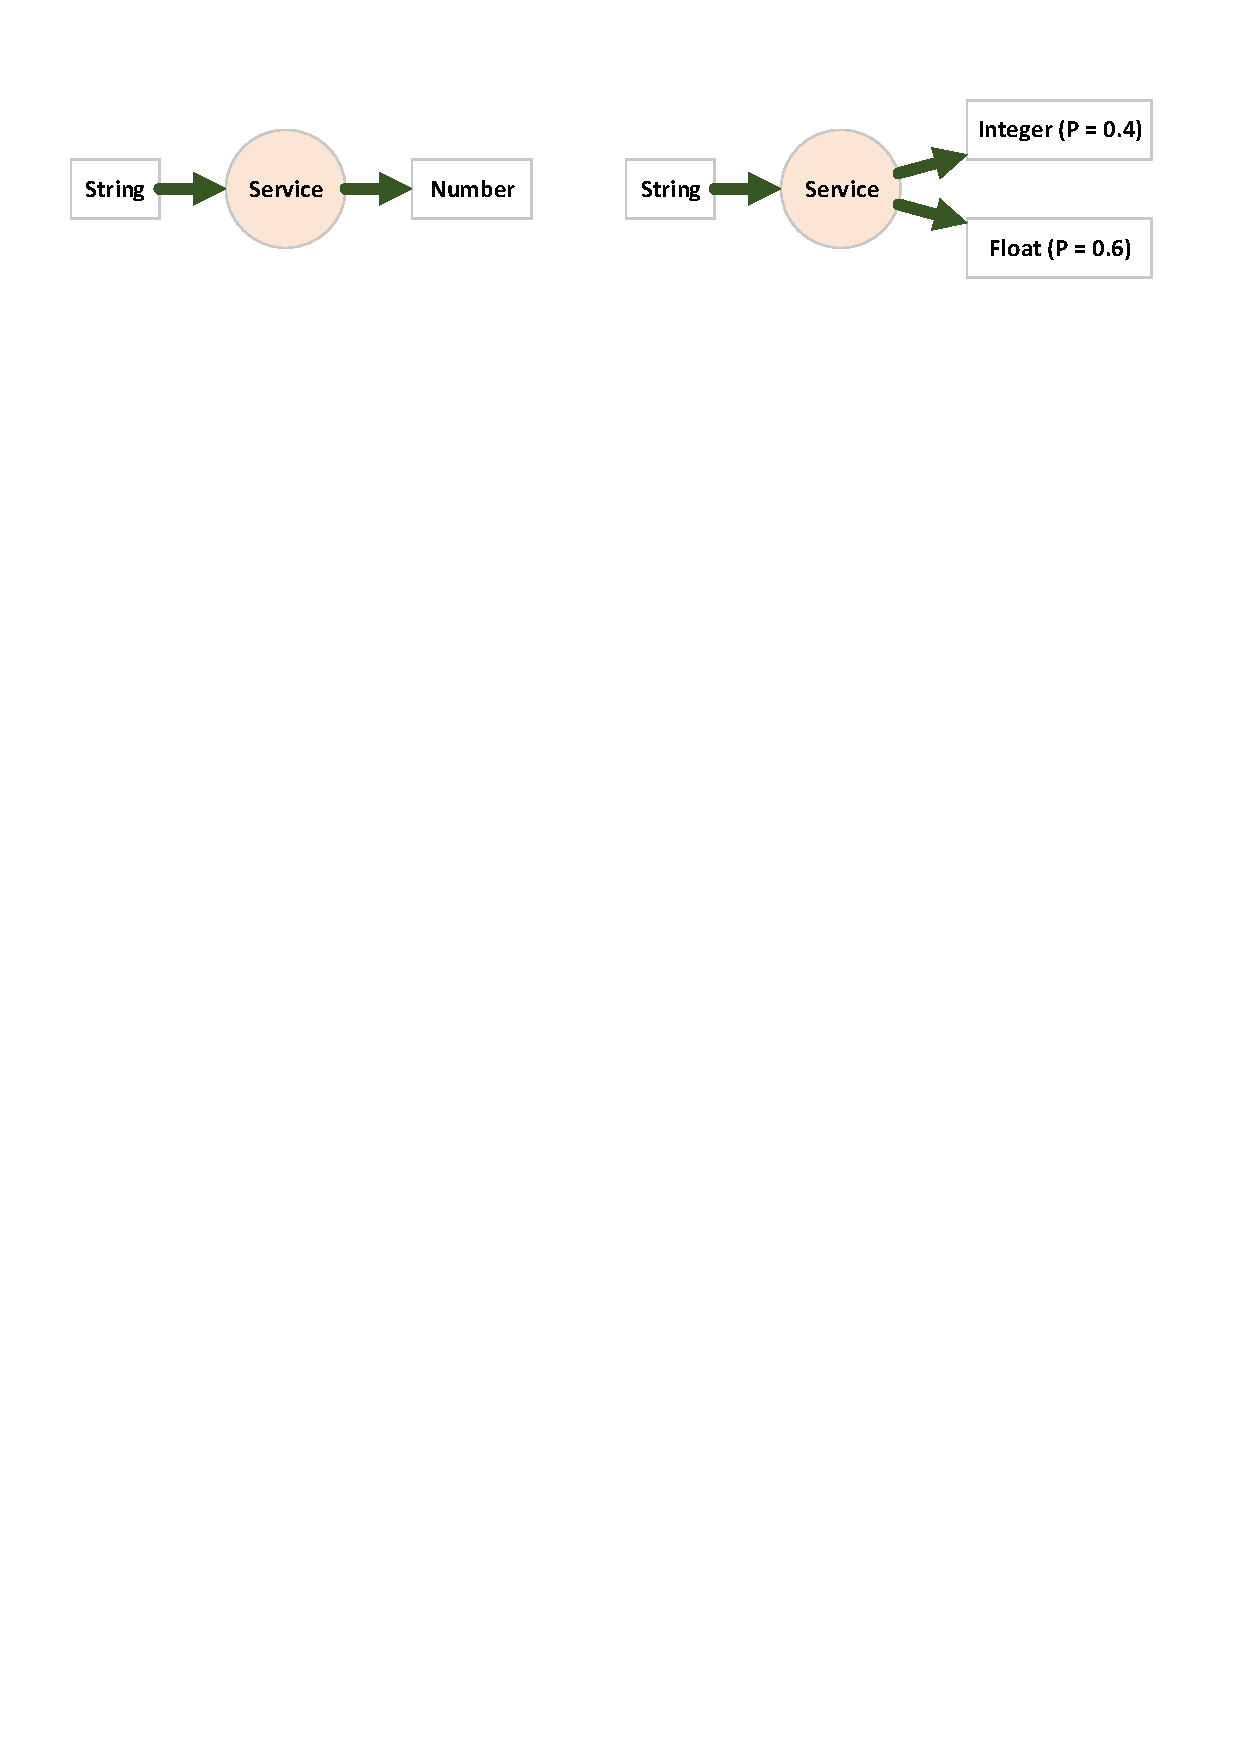
\includegraphics[width=9cm]{dataset_example.pdf}}

\vfill

Tasks requiring branching were created.

\end{frame}

\note{
  \begin{itemize}
   \item The datasets were created by extending WSC2008, a well-known dataset in the field. We chose WSC2008 because it is easily extendable to contain QoS values, and it already used an ontology of input and output values, meaning that services which produce a certain output type can be easily extended to produce two different output subtypes of the original.
   \item For example, if a service originally produces number, it can be changed to produce an integer 40\% of the time and a floating point number 60\% of the time.
   \item Services in the datasets were modified this way, with arbitrary probabilities which always add to 1.
   \item The original dataset tasks were also extended to require the use of branching.
  \end{itemize}
}

%------------------------------------------------

\begin{frame}
\frametitle{Results}

\begin{table}
\fontsize{4}{5.332}\selectfont
\centerline{
\def\arraystretch{1.5}
\begin{tabular}{c|c|c|}
\cline{2-3}
                                          & \multicolumn{2}{c|}{\textbf{Conditional}}      \\ \hline
\multicolumn{1}{|c|}{\textbf{Set (size)}} & \textbf{Avg. fitness} & \textbf{Avg. time (s)} \\ \hline
\multicolumn{1}{|c|}{1 (158)}                   & \cellcolor{blue!20} 0.601 $\pm$ 0.013      & \cellcolor{red!20} 1.290 $\pm$ 0.100    \\ \hline
\multicolumn{1}{|c|}{2 (558)}                   & 0.712 $\pm$ 0.009                          & 2.829 $\pm$ 0.250                        \\ \hline
\multicolumn{1}{|c|}{3 (604)}                   & 0.631 $\pm$ 0.008                          & 13.285 $\pm$ 1.229                       \\ \hline
\multicolumn{1}{|c|}{4 (1041)}                   & 0.718 $\pm$ 0.048                          & 6.146 $\pm$ 0.574                        \\ \hline
\multicolumn{1}{|c|}{5 (1090)}                   & 0.698 $\pm$ 0.005                          & 11.759 $\pm$ 0.948                       \\ \hline
\multicolumn{1}{|c|}{6 (2198)}                   & 0.662 $\pm$ 0.017                          & 92.392 $\pm$ 11.353                      \\ \hline
\multicolumn{1}{|c|}{7 (4113)}                   & 0.578 $\pm$ 0.010                          & 97.344 $\pm$ 13.705                      \\ \hline
\multicolumn{1}{|c|}{8 (8119)}                   & 0.656 $\pm$ 0.005                          & 326.387 $\pm$ 37.659                     \\ \hline
\end{tabular}
}
\end{table}

\begin{table}
 \fontsize{4}{5.332}\selectfont
\centerline{
\def\arraystretch{1.5}
\begin{tabular}{c|c|c|c|c|}
\cline{2-5}
                                          & \multicolumn{4}{c|}{\textbf{Non-conditional}}                                                                                                                                       \\ \cline{2-5} 
                                          & \multicolumn{2}{c|}{\textbf{If branch}}                                                  & \multicolumn{2}{c|}{\textbf{Else branch}}                                                \\ \hline
\multicolumn{1}{|c|}{\textbf{Set (size)}} & \multicolumn{1}{c|}{\textbf{Avg. fitness}} & \multicolumn{1}{c|}{\textbf{Avg. time (s)}} & \multicolumn{1}{c|}{\textbf{Avg. fitness}} & \multicolumn{1}{c|}{\textbf{Avg. time (s)}} \\ \hline
\multicolumn{1}{|c|}{1 (158)}             & \multicolumn{1}{c|}{\cellcolor{blue!20} 0.508 $\pm$ 0.000}     & \multicolumn{1}{c|}{\cellcolor{red!20} 0.563 $\pm$ 0.144}      & \multicolumn{1}{c|}{\cellcolor{blue!20} 0.588 $\pm$ 0.037}     & \multicolumn{1}{c|}{\cellcolor{red!20} 0.718 $\pm$ 0.079}      \\ \hline
\multicolumn{1}{|c|}{2 (558)}             & \multicolumn{1}{c|}{0.588 $\pm$ 0.084}     & \multicolumn{1}{c|}{1.490 $\pm$ 0.526}      & \multicolumn{1}{c|}{0.694 $\pm$ 0.016}     & \multicolumn{1}{c|}{1.527 $\pm$ 0.194}      \\ \hline
\multicolumn{1}{|c|}{3 (604)}             & 0.365 $\pm$ 0.000                          & 4.387 $\pm$ 0.768                           & 0.788 $\pm$ 0.000                          & 7.099 $\pm$ 0.906                           \\ \hline
\multicolumn{1}{|c|}{4 (1041)}            & 0.689 $\pm$ 0.064                          & 4.510 $\pm$ 1.177                           & 0.741 $\pm$ 0.429                          & 3.568 $\pm$ 0.429                           \\ \hline
\multicolumn{1}{|c|}{5 (1090)}            & 0.446 $\pm$ 0.000                          & 5.726 $\pm$ 0.755                           & 0.688 $\pm$ 0.011                          & 6.491 $\pm$ 0.743                           \\ \hline
\multicolumn{1}{|c|}{6 (2198)}            & 0.412 $\pm$ 0.063                          & 58.295 $\pm$ 12.765                         & 0.645 $\pm$ 0.024                          & 52.308 $\pm$ 5.785                          \\ \hline
\multicolumn{1}{|c|}{7 (4113)}            & 0.363 $\pm$ 0.000                          & 44.838 $\pm$ 5.926                          & 0.688 $\pm$ 0.032                          & 51.725 $\pm$ 4.260                          \\ \hline
\multicolumn{1}{|c|}{8 (8119)}            & 0.474 $\pm$ 0.000                          & 106.119 $\pm$ 7.152                         & 0.766 $\pm$ 0.002                          & 186.896 $\pm$ 20.008                        \\ \hline
\end{tabular}
}
\end{table}

\end{frame}

\note{
\begin{itemize}
 \item The results are divided into two tables, one for solutions with branching and the other for when the branches are individually produced.
 \item By comparing the two tables we see that two patterns arise: we see that the fitness value of the conditional solution is roughly equal to the average of the fitness values of the two separate branches, which potentially indicates that these solutions have a similar structure; we also see that the mean execution time for creating the conditional solution is roughly the sum of the mean times for each branch, showing that there is no performance slowdown for the creation of branched solutions.
 \item This is key finding which indicates that branched approach can be just as efficient as a non-branched one.
\end{itemize}

}

%------------------------------------------------
\section{Conclusions}
\subsection{}
%------------------------------------------------

\begin{frame}
\frametitle{Conclusions}
Novel approach addresses {\color{blue}three composition dimensions} simultaneously (fully functional, contain branches, quality-optimised).

\begin{itemize}
\item Solutions found with similar performance as non-branching technique.
\end{itemize}

\vfill

\setbeamercolor{postit}{fg=black,bg=cyan!20}
\begin{beamercolorbox}[sep=1em]{postit}
\textbf{Future work:} More than two branches, more complex branching conditions, analysis of convergence behaviour.
\end{beamercolorbox}
\end{frame}

\note{
\begin{itemize}
 \item In conclusion, in this work we have presented a GP approach capable of producing solutions that address three composition dimensions simultaneously: they are fully functional, support solutions with branching, and are optimised with regards to their quality of service attributes.
 \item Experiments showed that these solutions are generated with similar performance as that of a technique that does not support branching.
 \item In the future, we would like to extend this technique to handle more than two branches, as well as more complex branching conditions; finally, we would like to perform further experiments in order to analyse more thoroughly the convergence behaviour of our technique.
\end{itemize}

}

%------------------------------------------------

\begin{frame}
\Large
\centerline{Thank you!}
\medskip
\centerline{Questions\textcolor{red}{\textbf{?}}}
\end{frame}

\note{Thank you! Are there any questions?}

%----------------------------------------------------------------------------------------

\end{document} 